\documentclass[12pt,a4paper]{article}
\usepackage{geometry}
\usepackage[numbers]{natbib}
\usepackage{amssymb, amsmath}
\usepackage{graphicx}
\usepackage{grffile}
\graphicspath{{../Figures/}}
\usepackage{gensymb}
\usepackage[font=small]{caption}
\usepackage[utf8]{inputenc}
\usepackage[english]{babel}
\usepackage{fancyhdr}
\usepackage[raggedright]{titlesec}
\usepackage{subcaption}
\usepackage{multirow}
\usepackage{dirtytalk}
\usepackage{framed}
\usepackage[normalem]{ulem}
\usepackage[pdftex,breaklinks]{hyperref}
\hypersetup{
  colorlinks   = true, %Colours links instead of ugly boxes
  urlcolor     = green, %Colour for external hyperlinks
  linkcolor    = blue, %Colour of internal links
  citecolor   = red %Colour of citations
}


\begin{document}
\author{Katrina Ashton}


\pagestyle{fancy}
\fancyhf{}
\rhead{\thepage}
\lhead{u5586882}

\section{What I've done}
\begin{itemize}
\item Installed new SDK on TX1.
\item Did a bit more work on trying to get registration working for the external dataset.
%\item{Added more to the appendices for the final report draft}
\end{itemize}

\section{Parts of report to look at}
\begin{itemize}
\item{Sections 8-10 (basic outline right now)}
\end{itemize}

\section{Questions}
\begin{itemize}
\item
\end{itemize}

\section{Comments}
\begin{itemize}
\item Zheyu Zhuang wants to borrow the new RealSense for a few days. I'm going to lend it to him next week, and then hopefully he'll be done with it by Friday.
\item I had a look at the new depth image. It's much better quality-wise than the R200. However the RGB and depth images are not aligned, so getting corresponding pixels could be a bit tricky. I need to have a better look at their code to work out if that's part of the problem. (See Figure \ref{f: D415 offset}).
\item I think Pieter said that the new RealSense SDK is compatible with ROS, which might make aligning all of the time stamps a bit easier. I don't know the details but it's something to look into.
\item I haven't gotten around to installing ROS yet so I still haven't synched up the timestamps.
\item I've done a bit of work on trying to get the frames right for the registration, but probably still needs some work. 
\item I wrote up a more detailed explanation of the registration algorithms (see Section \ref{sec: algo}). Probably needs a bit more detail (especially theory/equations), so I'll try add some more this week.
\end{itemize}

\begin{figure}[t!]
  \centering
  \begin{subfigure}[t]{0.5\textwidth}
  \centering
    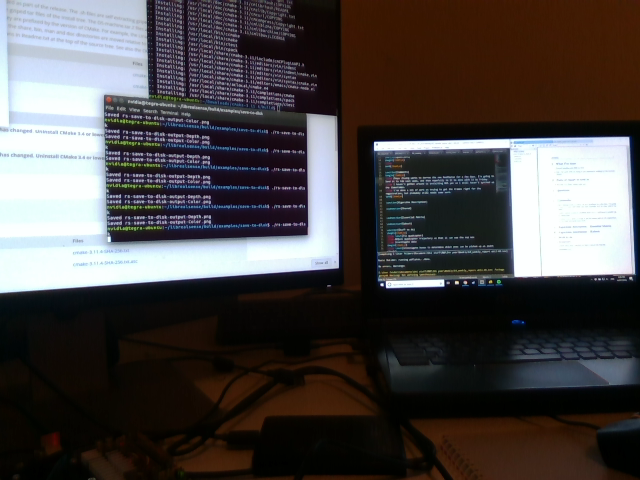
\includegraphics[width=60mm]{camera_tests/rs-save-to-disk-output-Color.png}
  \caption{Colour Image (640 x 480)}
  \end{subfigure}%
  ~
  \begin{subfigure}[t]{0.5\textwidth}
  \centering
    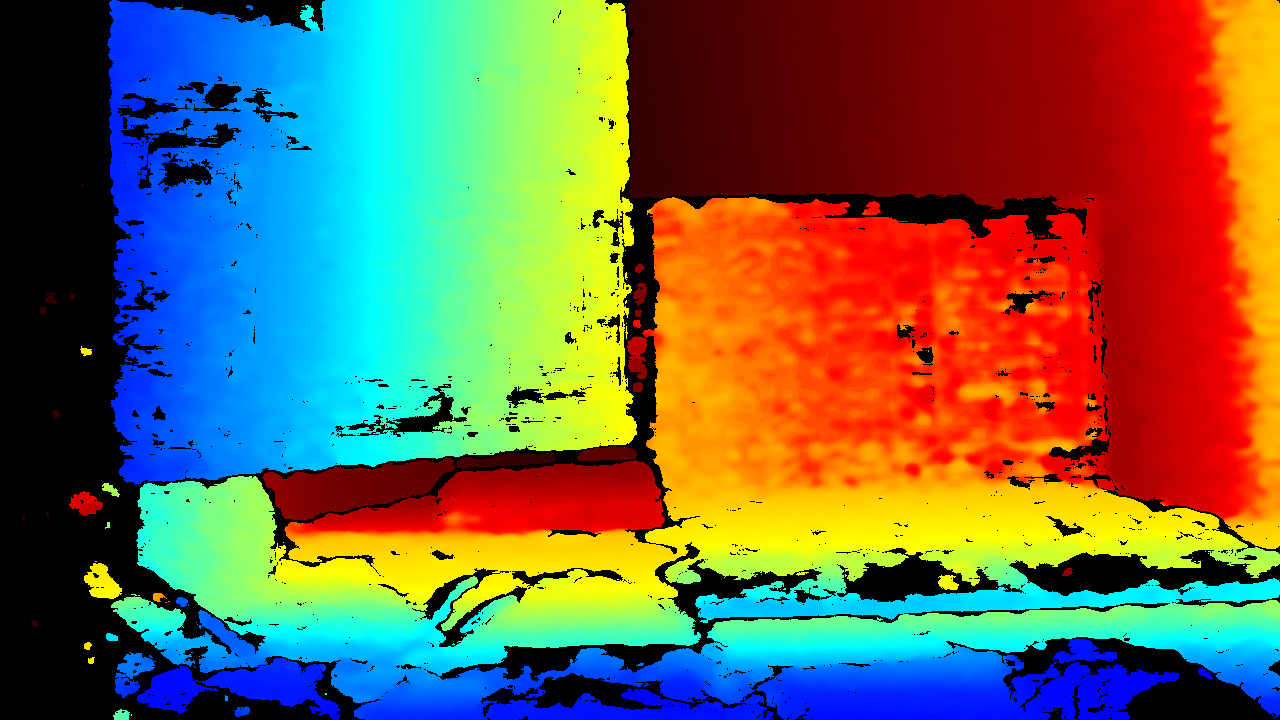
\includegraphics[width=60mm]{camera_tests/rs-save-to-disk-output-Depth.png}
  \caption{Depth Image (1280 x 720)}
  \end{subfigure}
  \caption{Images captured from RealSense RD415, note that the image dimensions are different and the depth image captures more of the scene to the right}
  \label{f: D415 offset}
\end{figure}

\section{Algorithm Description}
\label{sec: algo}

\subsection{Shared}
For each approach, the reconstructed trajectory of the camera is stored in two arrays: one with the x,y and z components of the position, and another with the w, x, z and z components of a Quaternion that gives the orientation. These formats were chosen as it is how the ground truth is stored.
\\\\
The initial position and orientation are initialized as the first values in the ground truth.
\\\\
Next, the frames are looped over. Right now the timestamps are not aligned, so I'm looping over the number of depth images as there are less of them. The following will describe what happens in each loop.
\\\\
The current RGB image and the one from the next timestamp are both loaded. The keypoints of each image are found using SIFT, they are then matched using a brute force method. The matches are then ordered in terms of their distance (i.e. how good a match they are). 
\\\\
The matches are then iterated over, and matches with a distance of less than 180 (found via trial and error) are kept. If there are less than 6 points the Essential Matrix cannot be found, so the loop is restarted with the next frame. If there are more than 6 points, two different methods are used to recover the camera pose: finding the Essential Matrix (see Section \ref{ssec: essential mat}), and aligning matched 3D points using Kabsch (see Section \ref{ssec: kabsch}).

\subsection{Essential Matrix}
\label{ssec: essential mat}
The Essential Matrix can be found in opencv using matched points and the focal length and principal point of the camera. Opencv can then be used to recover the pose difference between the two set of matched points using the above information and the Essential Matrix. I think this pose is given in the camera frame (before it moves) but I need to double check that I'm giving it the points in the right order.

\subsection{Kabsch}
\label{ssec: kabsch}
Once the matched points have been found, a depth needs to be associated with each one. Currently the pixel with the same indices as the RGB image is taken from the depth image. However upon inspecting the data more closely it seems like the RGB and depth images are not aligned, thus more processing will be necessary to find the corresponding point in the depth image.
\\\\
Once the corresponding depth has been found, a 3D point is defined with the $x$ and $y$ components from the RGB image width and height, respectively and the depth as the $z$ component. As these points are matched, the Kabsch algorithm can be used to align them.
\\\\
However, before this can be done the points need to be converted out of the image frame and into the camera frame. To do this, the following equations are used
\begin{align*}
z^c &= z^i /sf \\
x^c &= (x^i - cx)*z^c / fx \\
y^c &= (y^i - cy)*z^c / fy \\
\end{align*}
Where the superscript indicates the frame ($c$ for camera, $i$ for image), $sf$ is a scaling factor provided by the makers of the dataset, $cx$ and $cy$ are the $x$ and $y$ components of the optical center, and $fx$ and $fy$ are the $x$ and $y$ components of the focal length.
\\\\
Then Kabsch is applied. First, a $P$ and $Q$ matrix are defined, with each row being a point (first column $x$, second $y$, third $z$).The points are then centered, this is done by subtracting from each row in the matrix the centroid of that matrix. (The centroid is the sum of all the elements divided by the number of elements, done separately for each component). The translation is then given by the centroid of $Q$ minus the centroid of $P$.
\\\\
Next, the cross-covariance matrix, $H$, is found:
\[
H = P^T Q
\]
The rotation matrix from $P$ to $Q$ is given by 
\[
R = (H^TH)^{1/2}H^{-1}
\]
To actually calculate this, the singular value decomposition (SVD) is used:
\begin{align*}
H &= USV^T \\
d &= \text{det}(VU^T) \\
R &= V \begin{bmatrix} 1 & 0 & 0 \\ 0 & 1 & 0 \\ 0 & 0 & d \end{bmatrix} U^T
\end{align*}

\subsection{Updating global trajectory}
After the pose is acquired (as a translation and rotation matrix), the global trajectory needs to be updated. We have pose in the camera frame, so we can update the trajectories as follows:
\begin{align*}
Q_{m}^{g,n} &= Q_{m}^{g,n-1} * Q_{m}^{c,n} \\
P_{m}^{g,n} &= P_{m}^{g,n-1} + Q_{m}^{g,n-1}(P_{m}^{c,n})
\end{align*}

\noindent
Where $Q$ are the orientations (in quaternions), and $P$ are the positions. The subscript is for the method used for registration ($rgb$ for using only the RGB images via the Essential Matrix, and $d$ for also using the depth images via Kabsch). The superscript starts with the frame the measurement is in ($g$ for global, $c$ for camera, $i$ for image) and then gives the timestep the measurement is for (where $n$ is the current timestep).
\\\\
Note that the first position is not rotated, as it is already in the global frame. The second position is rotated, as it is in the camera frame (this is the translation found by registration). This position is rotated by the global rotation from the last timestep, as it is in the camera frame (i.e. with respect to the camera orientation at the end of the last timestep).


\section{Stuff to do}
\begin{itemize}
\item Adjust quadcopter trajectory so that it can see the top box
\item Write acquisition code for D415
\item Investigate data
\begin{itemize}
\item \sout{Investigate boxes to determine which ones can be picked up as point clouds}
\item \sout{Investigate RealSense cameras, compare the two cameras and using them on TX1/TX2 or Windows/Ubuntu}
\end{itemize}
\item Investigate registration algorithm
\begin{itemize}
\item Generate 3D object in MATLAB that I can get points from from various camera poses (may also need to get RGB and depth images if we're going with that approach?)
\item Apply registration algorithm to generated point clouds (ground truth known) -- without noise first, then add noise. Get error in true and estimated translation and rotation.
\end{itemize}
\item Try registration on external dataset
\begin{itemize}
\item Feature-only method (Essential Matrix)
\item Feature and depth method (Kabsch)
\item Install ROS and use it to align timestamps
\item Ensure that every pose is given with respect to the appropriate frame (ground truth is given in global frame, so each registered pose should be stored in global frame)
\item Incorporate IMU data
\end{itemize}
\item Reading
\begin{itemize}
\item \sout{Incorporating RGB and depth images -- feature matching (papers you sent me)}
\item Write up summary of main points (parts of the algorithm, choices with advantages/disadvantages)
\item See if more recent papers have made advancements
\end{itemize}
\end{itemize}

\end{document}